\documentclass[spanish, fleqn]{article}
\usepackage[spanish]{babel}
\usepackage[utf8]{inputenc}
\usepackage{amsmath}
\usepackage{amsfonts,txfonts}
\usepackage{mathrsfs}
\usepackage[colorlinks, urlcolor=blue]{hyperref}
\usepackage{fourier}
\usepackage[top = 2.5cm, bottom = 2cm, left = 2cm, right = 2cm]{geometry}
\usepackage{graphicx}
\usepackage{scalerel,stackengine}



\title{\textsc{Elementos de Análisis para Computación e Informática} \\
    \textsc{Examen Final}}

\author{Martín Villanueva}
\date{27 de Mayo 2016}

\begin{document}
\maketitle


\section*{\textsc{Tareas}}


\begin{description}

    \item[\textsc{Tarea 1.}] Sean $(X , \sigma)$ y $(X, \sigma')$ espacios métricos y \textit{quasimétricos} respectivamente. Denotemos a la topología generada/inducida por $\sigma$ por:
    \begin{align*}
        \mathcal{F} = \{ A \subset X: \ A \ \text{es un abierto, i.e:} \ \ \forall x \in A, \ \exists \delta>0: \ B_{\sigma}(x,\delta) \subset A \}
    \end{align*}
    donde adicionalmente sabemos que una base para esta topología es:
    \begin{align*}
        B = \{ B_{\sigma}(x, \sigma): \ x \in X, \ \delta \ \in \mathbb{R}_{0}^{+}  \}
    \end{align*}
    y también consideremos la siguiente \textit{posible} base para dicha topología:
    \begin{align*}
        B' = \{ B_{\sigma'}(x,\delta): \ x \in X, \ \delta \ \in  \mathbb{R}_{0}^{+} \cup \{ \infty \} \}
    \end{align*}
    se puede ver claramente que $B \subset B'$, pues $B'$ contiene los mismos miembros que $B$, más las bolas de radio infinito (\textit{que abarcan todo el espacio!}). Además como $B$ es una base para $\mathcal{F}$, cualquier abierto $\in \mathcal{F}$ puede escribirse como una reunión de miembros de $B$.

    Sea $\mathcal{A}$ un conjunto indexador (no necesariamente contable, ni finito), entonces cualquier reunión de bolas \newline $ \bigcup_{\alpha \in \mathcal{A}} B_{\alpha}  \ (B_{\alpha} \in B)$, puede formarse también con miembros de $B'$, pues $B \subset B'$.
    Consideremos ahora reuniones sobre $B'$. Si entre los miembros no hay bolas de radio infinito, el resultado es análogo
    al anterior. Consideremos entonces el caso de una reunión con al menos una bola de radio infinito $B_{\sigma'}(x_0, \infty)$:
    \begin{align*}
        \bigcup_{\alpha \in \mathcal{A}} B_{\alpha} \ (B_{\alpha} \in B') = B_{\sigma'}(x_0, \infty)
    \end{align*}
    tal resultado puede obtenerse por reuniones de miembros en $B$ como sigue:
    \begin{align*}
        \bigcup_{\delta > 0} B_{\sigma}(x_0, \delta)
    \end{align*}

    Luego, hemos probado que cada reunión de miembros en una base, puede formarse con los miembros de la otra (y viceversa). Por lo tanto ambas son bases de $\mathcal{F}$, y entonces $\sigma$ y $\sigma'$ generan/inducen la misma topología.




    \item[\textsc{Tarea 2.}] Se definen $(S,\sigma)$ un espacio métrico, el conjunto $E \neq \emptyset$, el conjunto de funciones $\mathcal{F}(E,S) = \left\{f: E \rightarrow S \right\}$, y la aplicación:
    \begin{align*}
        \Sigma(f,g) = \sup_{t \in E}\ \sigma \left(f(t),g(t)\right), \ \ \ \ \text{con} \ \ f,g \in \mathcal{F}(E,S),
    \end{align*}
    donde se quiere probar que $(\mathcal{F}(E,S),\Sigma)$ es un espacio \textit{quasimétrico}. Ya que $\sigma \left(f(t),g(t)\right)$ $(\forall t \in E)$ puede no estar acotado superiormente, entonces $\Sigma(f,g)$ puede ser infinita. Se verifica que $\Sigma$ cumple los axiomas usuales para una métrica, para $f,g,h \in \mathcal{F}(E,S$:
    \begin{enumerate}
         \item $\left(\Sigma(f,g) \geq 0 \right)$. Se sigue directamente desde el codominio de $\sigma : S \times S \rightarrow \mathbb{R}_0^+$.
         \item $\left(\Sigma(f,g) = 0 \leftrightarrow f=g \right)$. Como $\Sigma(f,g) = 0 \leftrightarrow \displaystyle \sup_{t \in E} \  \sigma\left(f(t), g(t) \right) = 0$, por la definición de supremo esto es equivalente a $\sigma\left( f(t), g(t) \right) \leq 0$. Ya que $\sigma$ es un métrica de $S$, la única posibilidad es que $\sigma\left(f(t),g(t)\right)=0 \leftrightarrow f(t) = g(t)$.
         \item $\left(\Sigma(f,g) = \Sigma(g,f) \right)$. Dada la simetría de la métrica $\sigma$, entonces:
         \begin{align*}
             \Sigma(f,g) = \sup_{t \in E} \ \sigma\left(f(t), g(t) \right) = \sup_{t \in E} \ \sigma\left(g(t), f(t) \right) = \Sigma(g,f).
         \end{align*}
         \item $\left(\Sigma(f,g) \leq \Sigma(f,h) + \Sigma(h,g) \right)$. Si se fija un $t_0 \in E$, luego para $f(t_0), g(t_0), h(t_0) \in S$ se cumple:
         \begin{align}
             \sigma\left(f(t_0), g(t_0) \right) \leq \sigma\left(f(t_0), h(t_0) \right) + \sigma\left(h(t_0), g(t_0) \right),
         \label{eq:triang}
         \end{align}
         pues $\sigma$ es métrica. Como (\ref{eq:triang}) es válida $\forall t_0 \in E$, entonces se verifica que:
         \begin{align*}
             \sup_{t\in E} \ \sigma\left(f(t), g(t) \right) \leq \sup_{t\in E} \ \sigma\left(f(t), h(t) \right) + \sup_{t\in E} \ \sigma\left(h(t), g(t) \right).
         \end{align*}
    \end{enumerate}
    Dado que $\Sigma: \mathcal{F}(E,S) \times \mathcal{F}(E,S) \rightarrow [0,\infty]$ y verifica los axiomas de métrica, entonces $\left(\mathcal{F}(E,S), \Sigma \right)$ es un espacio \textit{quasimétrico}.



    \item[\textsc{Tarea 3.}] Demostrar que $Z$ es cerrado en $\mathcal{F}(X,\mathbb{R})$, es equivalente a demostrar que $ Y = \mathcal{F}(X,\mathbb{R}) \setminus Z$ es abierto. Para cada $\phi \in Y$ y $\delta >0$ es posible definir las bolas abiertas:
    \begin{align*}
        B(\phi, \delta) = \left\{ \psi \in \mathcal{F}(X,\mathbb{R}): \Sigma(\phi,\psi) = \sup_{x \in X} |\phi(x)-\psi(x)| < \delta \right\}.
    \end{align*}
    Notar entonces lo siguiente:
    \begin{align*}
        \text{Si } \sup_{x \in X} |\phi(x)-\psi(x)| < \delta \ &\Leftrightarrow \ |\phi(x)-\psi(x)| < \delta \ \ \ \ \forall x \in X \\
        & \Leftrightarrow \phi(x)-\delta < \psi(x) < \phi(x)+\delta \ \ \ \ \forall x \in X.
    \end{align*}
    Si se fija $x$ en la última expresión, y se toma un $y \in X$ (también fijo) tal que $0 < d(x,y) <  \phi(x) - \psi(y)$, entonces se puede definir $\delta := \delta_{x,y} = \phi(x) - \psi(y) - d(x,y)$ el cual claramente es positivo, pero:
    \begin{align}
        \phi(x) - \delta = \phi(x) - (\phi(x) - \psi(y) - d(x,y) ) = d(x,y) + \psi(y) < \psi(x),
    \label{eq:break}
    \end{align}
    donde (\ref{eq:break}) es válido para todo $x,y \in X$ (fijos pero arbitrarios) que cumplan $0 < d(x,y) <  \phi(x) - \psi(y)$. Dado que no se satisface $\psi(x)-\psi(y) \leq d(x,y)$, entonces $\psi \notin Z$ y por tanto $\psi \in Y$. Ademas, puesto que:
    \begin{align*}
        \forall \phi \in Y, \ \exists \delta = \delta_{x,y} = \phi(x) - \psi(y) - d(x,y), \text{ con } 0 < d(x,y) <  \phi(x) + \psi(y), \text{ tal que } B(\phi, \delta) \subset Y, 
    \end{align*}
     se concluye que $Y$ es abierto, y por tanto $Z$ es cerrado. 





    \item[\textsc{Tarea 4.}] Veamos cada punto separadamente:
    \begin{enumerate}
        \item $\displaystyle \int_{\mathbb{R}} |\chi_{[-1,1]}(t)|\ dt = \int_{-1}^{1} |1| dt = 2 < \infty$, por lo tanto $\chi_{[-1,1]} \in L^1$.
        \item $\displaystyle \widehat{\chi_{[-1,1]}(t)} = \int_{\mathbb{R}} \chi_{[-1,1]}(t) e^{-2 \pi i \omega t} dt = \int_{-1}^{1} e^{-2 \pi i \omega t} dt$. Haciendo uso de la identidad de Euler:
        \begin{align*}
            \int_{-1}^{1} e^{i (-2 \pi \omega t)} dt = \int_{-1}^{1} \cos(-2 \pi \omega t) + i \sin(-2 \pi \omega t) dt
        \end{align*}
        tomando en cuenta la paridad de las funciones (\textit{y que la integral de una función impar en un intervalo simétrico es nula}):
        \begin{align*}
            \ldots = \int_{-1}^{1} \cos(2 \pi \omega t) dt - i \underbrace{\int_{-1}^{1} \sin(2 \pi \omega t) dt]}_{= 0 \ \text{por imparidad}} = \frac{\sin(2 \pi \omega t)}{2 \pi \omega} \bigg|_{-1}^{1} = \frac{\sin(2 \pi \omega)}{\pi \omega}
        \end{align*}
        \item Para probar que $\displaystyle \widehat{\chi_{[-1,1]}(t)} \notin L^1$, basta probar que $ \displaystyle \int_{-\infty}^{+\infty} \left|\widehat{\chi_{[-1,1]}(t)}(\omega)\right| d\omega$ diverge. Para ello se considera que:
        \begin{align*}
            \int_{-\infty}^{+\infty} \left|\widehat{\chi_{[-1,1]}(t)}(\omega)\right| d\omega \geq \int_{0}^{+\infty} \left|\widehat{\chi_{[-1,1]}(t)}(\omega)\right| d\omega.
        \end{align*}
        Dada la continuidad de $\displaystyle \widehat{\chi_{[-1,1]}(t)} = \frac{\sin(2 \pi \omega)}{\pi \omega}$, es posible hacer la siguiente descomposición:
        \begin{align*}
            \int_{0}^{+\infty} \left| \frac{\sin(2 \pi \omega)}{\pi \omega} \right| d\omega &= \lim_{n\rightarrow \infty} \sum_{k=1}^{n} \int_{k-1}^{k} \left|\frac{\sin(2 \pi \omega)}{\pi \omega}\right| d\omega \\
            &= \lim_{n\rightarrow \infty} \sum_{k=1}^{n} \int_{k-1}^{k} \frac{\left| \sin(2 \pi \omega) \right|}{\pi \omega} d\omega \\
            &\geq \lim_{n\rightarrow \infty} \sum_{k=1}^{n} \int_{k-1}^{k} \frac{\left| \sin(2 \pi \omega) \right|}{\pi k} d\omega \\
            &=  \frac{1}{\pi} \lim_{n\rightarrow \infty} \sum_{k=1}^{n} \frac{1}{k} \underbrace{\int_{k-1}^{k} \left| \sin(2 \pi \omega) \right| d\omega}_{= \frac{2}{\pi} \ \ (*)} \\
            &= \frac{2}{\pi^2} \lim_{n\rightarrow \infty} \sum_{k=1}^{n} \frac{1}{k} = \infty,
        \end{align*}
        donde $(*)$ resulta de integrar $|\sin(2 \pi w)|$ sobre un periodo cualquiera de la función, y la divergencia proviene de la divergencia de la serie harmónica.


    \end{enumerate}




    \item[\textsc{Tarea 5.}] Veamos por partes:
    \begin{enumerate}
        \item Denotemos como $\displaystyle f(t)=e^{-t^2}$ y $\displaystyle g(t)=(1+t^2)^{-1}$. En primer lugar, es fácil notar que las derivadas de $f(t)$ son la misma función multiplicadas por un polinomio (\textit{regla de la cadena}). Cada nueva derivada aumenta en un grado el grado del polinomio respectivo, pues la derivada del exponente es $-2t$.
        Luego se puede escribir $f^{(n)}(t)=f(t)P_n(t)$, con $P_n$ el polinomio de grado $n$ respectivo. Entonces:
        \begin{align*}
            \lim_{|t|\rightarrow \infty} t^p D^q f(t) = \lim_{|t|\rightarrow \infty} t^p P_q(t) f(t) = \lim_{|t|\rightarrow \infty} \widehat{P}_{p+q}(t) f(t) = \lim_{|t|\rightarrow \infty} \frac{\widehat{P}_{p+q}(t)}{e^{t^2}} = 0 \ \ \ \forall \ p,q \in \mathbb{N}_0,
        \end{align*}
        lo último debido a que la exponencial crece más rápido que cualquier polinomio en $t \rightarrow \infty$. En segundo lugar, para probar que $g \notin \mathcal{C}^{\infty}(\mathbb{R},\mathbb{C})$, basta mostrar que existe alguna combinación de $p,q \in \mathbb{N}_0$ tales que $t^p D^q g(t) \rightarrow 0$ no se satisface. Veamos para $p=3$ y $q=1$:
        \begin{align*}
            \lim_{|t|\rightarrow \infty} \frac{t^3}{1+t^2} \rightarrow \infty,
        \end{align*}
        lo que completa la demostración.

        \item Utilizando la notación de multi-índices para $\alpha,\beta \in \mathbb{N}_0^n$, se quiere probar que los siguientes dos conjuntos:
        \begin{align}
            \mathcal{C}_{\downarrow}^{\infty}(\mathbb{R}^n,\mathbb{C}) &= \left\{ f \in \mathcal{C}^{\infty}(\mathbb{R}^n,\mathbb{C}): x^{\alpha} D^{\beta} f(x) \rightarrow 0, \ \ \text{cuando} \ \ ||x||_2 \rightarrow 0, \ \ \ \forall \alpha,\beta \in \mathbb{N}_0^n \right\} \label{eq:def1} \\
            \mathcal{S}(\mathbb{R}^n,\mathbb{C}) &= \left\{ f \in \mathcal{C}^{\infty}(\mathbb{R}^n,\mathbb{C}): ||f ||_{\alpha, \beta} = \sup_{x \in \mathbb{R}^n} \left|x^{\alpha} D^{\beta} f(x)\right| < \infty, \ \ \ \forall \alpha,\beta \in \mathbb{N}_0^n \right\} \label{eq:def2}
        \end{align}
        corresponden a definiciones equivalentes del mismo conjunto. Partamos de $\mathcal{C}_{\downarrow}^{\infty}(\mathbb{R}^n,\mathbb{C})$. Desde la definición del límite, notar que $\forall \epsilon$ existe un $M(\epsilon)$ tales que:
        \begin{align*}
            | x^{\alpha} D^{\beta} f(x)| < \epsilon, \ \ \text{cuando} \ \ ||x||_2 < M(\epsilon).
        \end{align*}
        Adicionalmente puesto que  $x^{\alpha} D^{\beta} f$ es continua en $[-M,M]$, por el Teorema de Weierstrass \cite{Weier}, esta debe alcanzar su máximo en tal intervalo. Entonces:
        \begin{align*}
            |x^{\alpha} D^{\beta} f(x)| \leq \max \left\{ \epsilon, \max_{x\in [-M(\epsilon),M(\epsilon)]} x^{\alpha} D^{\beta} f(x) \right\} < \infty, \ \ \ \forall x \in \mathbb{R}^n,
        \end{align*}
        que es equivalente a (\ref{eq:def2}). Partamos ahora de $\mathcal{S}(\mathbb{R}^n,\mathbb{C})$ (el cual existe y es finito). En primer lugar, denotemos a $\displaystyle \sup_{x \in \mathbb{R}^n} \left|x^{\alpha} D^{\beta} f(x)\right| = C_{\alpha,\beta}$. Si se define $\alpha+1 =(\alpha_1+1, \alpha_2+2, \cdots, \alpha_n+1)$, entonces:
        \begin{align*}
            {Si} \ \ \  \sup_{x \in \mathbb{R}^n} \left|x^{\alpha+1} D^{\beta} f(x)\right| < \infty
            \Rightarrow \left|x^{\alpha+1} D^{\beta} f(x)\right| \leq C_{\alpha+1,\beta} < \infty
            \Rightarrow  \left|x^{\alpha} D^{\beta} f(x)\right| \leq \frac{C_{\alpha+1,\beta}}{|x_1 \cdots x_n|},
        \end{align*}
        para todo $x \in \mathbb{R^n}$. Y luego (usando el Teorema de Acotamiento \cite{Squeeze}):
        \begin{align*}
            \lim_{||x||_2 \rightarrow 0} \frac{C_{\alpha+1,\beta}}{|x_1 \cdots x_n|} = 0 \Longrightarrow x^{\alpha} D^{\beta} f(x)\rightarrow 0 \ \ \ \text{cuando} \ \ \ ||x||_2\rightarrow 0,  \ \ \ \forall \alpha,\beta \in \mathbb{N}_0^n,
        \end{align*}
        que es la la definición en (\ref{eq:def1}).

        \item Se quiere probar que $\mathcal{S}(\mathbb{R}^n,\mathbb{C})$ es un espacio normado completo. Para ello se definen las operaciones $(+,\cdot)$ de forma usual, dando estructura de espacio vectorial a $\displaystyle \left(\mathcal{S}(\mathbb{R}^n,\mathbb{C}),+,\cdot \right)$. Se verifica en primer lugar que $||\cdot||_{\alpha,\beta}$ es una norma ($a \in \mathbb{C}$, y $f,g \in \mathcal{S}(\mathbb{R}^n,\mathbb{C})$):
        \begin{enumerate}
            \item $\left( ||a \cdot f||_{\alpha,\beta} = |a| \ ||f||_{\alpha,\beta} \right)$. Sigue directamente de la definición:
            \begin{align*}
                ||a \cdot f||_{\alpha,\beta} = \sup_{x \in \mathbb{R}^n} \left| x^{\alpha} D^{\beta} a f(x) \right| = \sup_{x \in \mathbb{R}^n} \left| a x^{\alpha} D^{\beta} f(x) \right| = |a| \sup_{x \in \mathbb{R}^n} \left| x^{\alpha} D^{\beta} f(x) \right| = |a| \ ||f||_{\alpha,\beta}
            \end{align*}
            \item $\left( ||f+g||_{\alpha,\beta} \leq ||f||_{\alpha,\beta} + ||g||_{\alpha,\beta }\right)$. Sigue directamente de la linealidad de la derivada $D^{\beta}$:
            \begin{align*}
                 ||f+g||_{\alpha,\beta} =  \sup_{x \in \mathbb{R}^n} \left| x^{\alpha} D^{\beta}\left( f(x)+g(x) \right) \right| &= \sup_{x \in \mathbb{R}^n} \left| x^{\alpha} D^{\beta} f(x) +  x^{\alpha} D^{\beta} g(x) \right| \\ &\leq \sup_{x \in \mathbb{R}^n} \left\{ \left| x^{\alpha} D^{\beta} f(x) \right| +  \left|  x^{\alpha} D^{\beta} g(x) \right| \right\}\\ &= \sup_{x \in \mathbb{R}^n}  \left| x^{\alpha} D^{\beta} f(x) \right| + \sup_{x \in \mathbb{R}^n}  \left|  x^{\alpha} D^{\beta} g(x) \right| = ||f||_{\alpha,\beta} + ||g||_{\alpha,\beta }
            \end{align*}
            \item $\left( ||f||_{\alpha,\beta}=0 \Leftrightarrow f \equiv 0 \right)$. Esta requiere un poco más de tratamiento. Notar que $||f||_{\alpha,\beta}=0 \Leftrightarrow x^{\alpha}D^{\beta} f(x) = 0 \ \ \forall x \in \mathbb{R}^n$. Luego para todo $x \neq \mathbf{0}$ se debe cumplir $D^{\beta} f(x)=0$, y dada la continuidad de $f \in \mathcal{S}(\mathbb{R}^n,\mathbb{C}) \subset C^{\infty}(\mathbb{R}^n,\mathbb{C})$, entonces $D^{\beta} f(x)=0 \ \ \forall x \in \mathbb{R}^n$ y se deduce que $f$ tiene estructura polinomial. Ya que $f(x)\rightarrow 0$ para $||x||_2 \rightarrow \infty$, la única posibilidad es que $f \equiv 0$.
        \end{enumerate}

        Para la completitud, notar que $\mathcal{S}(\mathbb{R}^n, \mathbb{C})$ es un espacio de funciones que mapea $\mathbb{R}^n \rightarrow \mathbb{C}$, y puesto que $(\mathbb{C},|\cdot|)$ es un espacio métrico completo  (\textit{isomorfo} a $\left(\mathbb{R}^2,|\cdot|\right)$), entonces $\mathcal{S}(\mathbb{R}^n, \mathbb{C})$ debe serlo también (\textbf{Lema 2.} de guía). Verifiquemos de todos modos. Se definen sucesiones de Cauchy $\{f_k \}$ de funciones $f_k \in \mathcal{S}(\mathbb{R}^n,\mathbb{C})$ con respecto a la métrica inducida por $||\cdot||_{\alpha,\beta}$, i.e:
        \begin{align}
          \forall \epsilon, \exists N \in \mathbb{N}\ \text{ tal que } \ \forall p,q > N: \ \ ||f_p-g_q||_{\alpha,\beta} < \epsilon \ \ \Leftrightarrow \sup_{x \in \mathbb{R}^n} |x^{\alpha}D^{\beta}(f_p(x)-f_q(x))|< \epsilon.
        \label{eq:SC}
        \end{align}
        Se debe verificar que $\{f_k \}$ converge en el mismo $\mathcal{S}(\mathbb{R}^n,\mathbb{C})$. Para ello se fijan múlti-índices $(\alpha, \beta)$ y $x \in \mathbb{R}^n$ (de forma arbitraria), y se nota lo siguiente:
        \begin{align*}
        	\left| x^{\alpha} D^{\beta} \left(f_p(x) - f_q(x) \right) \right| &< \epsilon \\
        	\left| x^{\alpha} D^{\beta} f_p(x) - x^{\alpha} D^{\beta} f_q(x) \right| &< \epsilon \ \ \ \ \ \ \ \forall p,q > N.
        \end{align*}
        De lo anterior es importante observar que si $f \in \mathcal{S}(\mathbb{R}^n, \mathbb{C})$, entonces $x^{\alpha} D^{\beta} f \in \mathcal{S}(\mathbb{R}^n, \mathbb{C})$,  luego $\left\{ x^{\alpha} D^{\beta} \left(f_k(x)\right) \right\}$ es una sucesión de Cauchy en $\mathbb{C}$, y por lo tanto debe existir una función $f \in \mathcal{S}(\mathbb{R}^n, \mathbb{C})$ tal que:
        \begin{align}
        	x^{\alpha}D^{\beta} f(x) := \ \lim_{k \rightarrow \infty} x^{\alpha}D^{\beta}f_k(x) \ \ \ \forall \alpha,\beta  \in \mathbb{N}_0^n \ \ \forall x \in \mathbb{R}^n.
        \end{align}
        Lo anterior no basta para deducir la \textit{convergencia uniforme}. Para ello se procede como sigue, haciendo uso de (\ref{eq:SC}):
        \begin{align*}
        	\left| x^{\alpha} D^{\beta} f_p(x) - x^{\alpha}D^{\beta} f(x) \right| &= \left| x^{\alpha} D^{\beta} f_p(x) - \lim_{q \rightarrow \infty} x^{\alpha}D^{\beta} f_q(x) \right| \\
        	&= \lim_{q \rightarrow \infty} \left| x^{\alpha} D^{\beta} \left( f_p(x) - f_q(x) \right) \right| \\
        	&\leq \lim_{q \rightarrow \infty} \sup_{x \in \mathbb{R}^n} \left| x^{\alpha} D^{\beta} \left( f_p(x) - f_q(x) \right) \right| \\
        	&=  \lim_{q \rightarrow \infty} ||f_p - f_q ||_{\alpha,\beta}  \\
        	&= ||f_p - f ||_{\alpha,\beta} < \epsilon.
        \end{align*}
        Dado que $\epsilon > 0$ es arbitrario, resulta que $f_p \rightarrow f$ con respecto a $||\cdot||_{\alpha,\beta}$ para $p \rightarrow \infty$, que es lo que se quería probar.



        \item Sean $f,g  \in \mathcal{S}(\mathbb{R},\mathbb{C})$. Verifiquemos en primer lugar que $f\cdot g \in \mathcal{S}(\mathbb{R},\mathbb{C})$. Para ello se hace uso de la \textit{regla generalizada de Leibniz} \cite{Leibniz}:
        \begin{align}
            D^n \left(f(t)g(t) \right) = \sum_{k=0}^n {n \choose k} f^{(k)}(t) g^{(n-k)}(t)
        \label{eq:leibniz}
        \end{align}
        Ocupando ahora (\ref{eq:leibniz}), se verifica la definición (\textit{equivalente}) de $\mathcal{S}(\mathbb{R},\mathbb{C})$:
        \begin{align*}
            \lim_{|t|\rightarrow \infty} t^p D^q \left( f(t)g(t) \right)
            &= \lim_{|t|\rightarrow \infty} t^p \sum_{k=0}^q {q \choose k} f^{(k)}(t) g^{(q-k)}(t) \\
            &= \lim_{|t|\rightarrow \infty} \sum_{k=0}^q {q \choose k} t^p f^{(k)}(t) g^{(q-k)}(t) \\
            &\stackrel{\text{(\#)}}{=} \sum_{k=0}^q {q \choose k}\lim_{|t|\rightarrow \infty}  \underbrace{t^p f^{(k)}(t)}_{\rightarrow 0} \underbrace{g^{(q-k)}(t)}_{\rightarrow 0} = 0 \ \ \ \ \ \forall p,q \in \mathbb{N}_0,
        \end{align*}
        donde (\#) es posible pues cada límite existe, y además son nulos pues $f^{(k)},g^{(q-k)} \in \mathcal{S}(\mathbb{R},\mathbb{C})$.

        Para verificar que $f * g \in \mathcal{S}(\mathbb{R},\mathbb{C})$, se toman en cuenta tres resultados: 1) Que el producto $f \cdot g \in \mathcal{S}(\mathbb{R},\mathbb{C})$ (recien probado), 2) Que la transformada de Fourier mapea $\mathcal{S}(\mathbb{R},\mathbb{C})$ en sí mismo (resultado de \textsc{Tarea 6.}), y 3) lo siguiente:
        \begin{align*}
            \widehat{f * g}(\omega) &= \int_{\mathbb{R}} \left( \int_{\mathbb{R}} f(y) g(x-y) dy \right) e^{-2 \pi i \omega x} dx \\
            &= \int_{\mathbb{R}} \left( \int_{\mathbb{R}} f(y) g(x-y) e^{-2 \pi i \omega x} dy \right) dx \\
            &=  \int_{\mathbb{R}} \left( \int_{\mathbb{R}} f(y) g(x-y) e^{-2 \pi i \omega x} dx \right) dy \\
            &= \int_{\mathbb{R}} \left( \int_{\mathbb{R}} g(x-y) e^{-2 \pi i \omega x} dx \right) f(y) dy \ \ \ \ (z = x-y) \\
            &= \int_{\mathbb{R}} \left( \int_{\mathbb{R}} g(z) e^{-2 \pi i \omega (z+y)} dz \right) f(y) dy \\
            &= \int_{\mathbb{R}} \left( \int_{\mathbb{R}} g(z) e^{-2 \pi i \omega z} dz \right) f(y) e^{-2 \pi i \omega y} dy \\
            &= \int_{\mathbb{R}} f(y) e^{-2 \pi i \omega y} dy \cdot \int_{\mathbb{R}} g(z) e^{-2 \pi i \omega z} dz = \widehat{f}(\omega) \cdot \widehat{g}(\omega).
        \end{align*}
        Entonces como $f,g \in  \mathcal{S}(\mathbb{R},\mathbb{C}) \Rightarrow \widehat{f},\widehat{g} \in  \mathcal{S}(\mathbb{R},\mathbb{C})$, y luego $\widehat{f * g} = \widehat{f}\cdot \widehat{g} \in  \mathcal{S}(\mathbb{R},\mathbb{C})$, se concluye lo pedido.

        \item En primer lugar, notar que para que una función $f$ (integrable) pertenezca al espacio $L^p(\mathbb{R}, \mathbb{C})$, debe satisfacer:
        \begin{align*}
             ||f||_{L^p} = \left( \int_{\mathbb{R}} |f(x)|^p dx \right)^{\frac{1}{p}} < \infty  \ \ \ \text{para } 1 \leq p < \infty.
        \end{align*}
        Se procede entonces mediante la siguiente construcción:
        \begin{align*}
            \int_{\mathbb{R}} \left|f(x)\right|^p dx = \int_{\mathbb{R}} \left((1+x^2)|f(x)|\right)^p\frac{1}{(1+x^2)^p} dx.
        \end{align*}
        Dado que $f  \in \mathcal{S}(\mathbb{R},\mathbb{C})$ entonces  $(1+x^2)f(x)$ está acotado, y $\displaystyle \frac{1}{(1+x^2)^p} \leq \frac{1}{1+x^2} \in L^1(\mathbb{R}, \mathbb{C}) \ \text{para } p\geq 1 $. Entonces:
        \begin{align*}
            \int_{\mathbb{R}} |f(x)|^p dx \leq ||f||_{2,0}^p \int_{\mathbb{R}} \frac{1}{1+x^2} dx < \infty,
        \end{align*}
        donde $\displaystyle \|f\|_{\alpha,\beta} = \underset{x\in\mathbb{R}^n}{\sup} |x^\alpha D^\beta f(x)|$. El caso $p = \infty$ se sigue directamente de  $f \in \mathcal{S}(\mathbb{R},\mathbb{C})$:
        \begin{align*}
             ||f||_{L^\infty} = \sup_{x \in \mathbb{R}} \left|f(x)\right| < \infty.
         \end{align*}
         Otra forma de \textit{entender} porqué esta inclusión es verdad es el siguiente argumento: Para cada función $f \in L^p(\mathbb{R})$ existe una función \textit{por partes} $h_n$, tal que $||h_n(x) - f(x)||_{2} \rightarrow 0 \ \text{con} \ n\rightarrow \infty \ (\forall x \text{ i.e. convergencia puntual})$ y entonces $||h_n - f||_{L^p} \rightarrow 0$ para $n \rightarrow \infty$. Dado que $h_n$ puede ser \textit{continuamente aproximada} por funciones de soporte compacto \textit{suaves} ($C_{c}^{\infty}(\mathbb{R})$), y que $C_{c}^{\infty}(\mathbb{R})$ es denso en $\mathcal{S}(\mathbb{R})$, entonces se concluye $\mathcal{S}(\mathbb{R}) \subset L^p(\mathbb{R})$.
    \end{enumerate}




    \item[\textsc{Tarea 6.}] Sea $f \in \mathcal{C}_{\downarrow}^\infty(\mathbb{R},\mathbb{C})$, se quiere demostrar que:
    \begin{align}
        (2 \pi i \gamma)^p D^q \widehat{f}(\gamma) = \left[D^p (-2 \pi i x)^q f(x)\right]\widehat{} \ \ \ \ \ \forall p,q \in \mathbb{N}_0.
    \label{eq:teo}
    \end{align}
    Para ello se definen las siguientes dos proposiciones:
    \begin{align*}
        \mathbf{P}_1(p) &: \ \ (2 \pi i \gamma)^p \widehat{f}(\gamma) = \left[D^p f(x) \right]\widehat{} \ \ \ \ \ \ \ \forall p \in \mathbb{N}_0 \\
        \mathbf{P}_2(q) &: \ \ D^q \widehat{f}(\gamma) = [(-2 \pi i x)^q f(x)]\widehat{} \ \ \ \ \ \forall q \in \mathbb{N}_0,
    \end{align*}
    cuyos casos bases (derivados en \cite{DymMcKean}) son respectivamente:
    \begin{align}
        (p=1) &: \ \ (2 \pi i \gamma) \widehat{f}(\gamma) = \left[ D f(x) \right]\widehat{} \label{eq:base1} \\
        (q=1) &: \ \ D \widehat{f}(\gamma) =  \left[ (-2 \pi i x) f(x) \right]\widehat{} \label{eq:base2}.
    \end{align}
    Probemos cada una por inducción. Para $\mathbf{P}_1$ se tiene:
    \begin{align*}
        (2 \pi i \gamma)^{p+1} \widehat{f}(\gamma) &= (2 \pi i \gamma)(2 \pi i \gamma)^{p} \widehat{f}(\gamma) \\
        &= (2 \pi i \gamma) \left[ D^p f(x) \right]\widehat{} \\
        &\stackrel{\text{(\#)}}{=} \ \ \left[ D(D^p f(x)) \right]\widehat{} \\
        & = \left[ D^{p+1} f(x) \right]\widehat{},
    \end{align*}
    donde en (\#) se usó la hipótesis inductiva (\ref{eq:base1}). Se procede de igual modo para $\mathbf{P}_2$:
    \begin{align*}
        D^{q+1} \widehat{f}(\gamma) &= D\left[D^{q} \widehat{f}(\gamma)\right] \\
        &= D_{\gamma} \left[(-2 \pi i x)^q f(x) \right]\widehat{} \\
        &\stackrel{\text{(\#)}}{=} \ \ \left[(-2 \pi i x)\ (-2 \pi i x)^q f(x) \right]\widehat{} \\
        &= \left[(-2 \pi i x)^{q+1} f(x) \right]\widehat{},
    \end{align*}
    donde en (\#) se uso la hipótesis inductiva (\ref{eq:base2}). Como $\mathbf{P}_1(p)\Rightarrow \mathbf{P}_1(p+1)$,
    y $\mathbf{P}_2(q) \Rightarrow \mathbf{P}_2(q+1)$, se han demostrado entonces ambas proposiciones. Luego, se puede proceder como sigue:
    \begin{align*}
        (2 \pi i \gamma)^p D^q \widehat{f}(\gamma) \ \ \stackrel{\mathbf{P}_2}{=} \ \ (2 \pi i \gamma)^p \left[ (-2 \pi i x)^q f(x) \right]\widehat{} \ \ \stackrel{\mathbf{P}_1}{=} \ \ \left[ D^p (-2 \pi i x)^q f(x) \right]\widehat{}\ \ ,
    \end{align*}
    lo que completa la prueba de (\ref{eq:teo}).

    Para la segunda parte, notar que aplicando valor absoluto a (\ref{eq:teo}) se obtiene:
    \begin{align*}
        \left|\gamma^p D^q \widehat{f}(\gamma)\right| &= \frac{1}{(2 \pi)^p} \left| \int_{\mathbb{R}} (-2 \pi i)^q D_{x}^{p} x^q e^{-2 \pi i \gamma x} dx \right| \\
        &\leq (2 \pi)^{q-p} \int_{\mathbb{R}} \left| D_{x}^{p} x^q f(x) \right| dx \\
        &= (2 \pi)^{q-p} \ \ ||D_{x}^p x^q f(x)||_{L^1} < \infty,
    \end{align*}
    puesto que $f \in \mathcal{C}_{\downarrow}^\infty(\mathbb{R},\mathbb{C}) \Rightarrow  D^p x^q f \in \mathcal{C}_{\downarrow}^\infty(\mathbb{R},\mathbb{C})$ y que $\mathcal{C}_{\downarrow}^\infty(\mathbb{R},\mathbb{C}) \subset L^1(\mathbb{R},\mathbb{C})$. Entonces como $\widehat{f} \in \mathcal{C}^\infty(\mathbb{R},\mathbb{C})$ y satisface $\left|\gamma^p D^q \widehat{f}(\gamma)\right| < \infty$, se concluye que $\widehat{f} \in \mathcal{C}_{\downarrow}^\infty(\mathbb{R},\mathbb{C})$, i.e, la transformada de Fourier mapea $\mathcal{C}_{\downarrow}^\infty(\mathbb{R},\mathbb{C})$ en sí mismo.




 
    \item[\textsc{Tarea 7.}] Se listan a continuación algunos ejemplos de funciones $f \in \mathcal{C}_{C}^{\infty}(\mathbb{R},\mathbb{C})$ (la extensión a varias variables se muestra a continuación):
    \begin{enumerate}
        \item Un ejemplo clásico es la función \textit{bump}, definida como:
        \begin{align*}
        \psi(x) =
        \begin{cases}
        e^{\frac{1}{x^2-1}} & |x|<1 \\
        0 & |x|>= 1,
        \end{cases}    
        \end{align*}
        cuya gráfica se ve en Figura \ref{fig:cbump}. Esta puede ser fácilmente extendida a otros intervalos de compacidad:
        \begin{align*}
        \widehat{\psi}(x) =
        \begin{cases}
        e^{\frac{1}{(x-a)^2-1}} & |x|<r \\
        0 & |x|>= r,
        \end{cases}    
        \end{align*}
        que tiene soporte compacto en $[a-r, a+r]$ con $a,r \in \mathbb{R}$.

    \begin{figure}[htpb!]
    \centering
    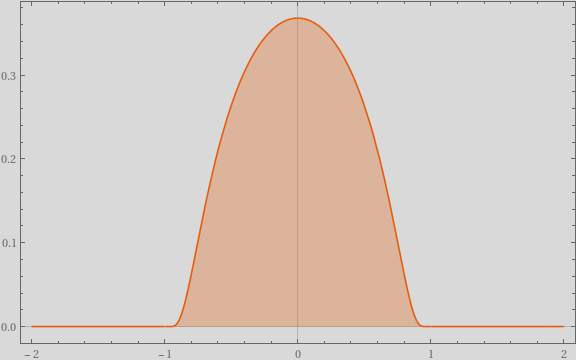
\includegraphics[width=10cm]{bump}
    \caption{Gráfico de función \textit{bump} clásica.}
    \label{fig:cbump}
    \end{figure}

    \item Otra construcción interesante considera a la función $\displaystyle f(x) = e^{\frac{-1}{x}}$, cuya ``gracia'' es que está en $\mathcal{C}^{\infty}(\mathbb{R})$ y $f(0)=0$. Con esta es posible definir:
    \begin{align}
        \phi(x) = \frac{f(x)}{f(x)-f(1-x)}
    \label{eq:trick}
    \end{align}
    la cual tambien pertenece a $\mathcal{C}^{\infty}(\mathbb{R})$, pero ademas $\phi(0)=0$ y $\phi(1)=1$. Entonces una función de soporte compacto se puede construir como sigue:
    \begin{align*}
        \psi(x) =
        \begin{cases}
        0 & x \leq 0 \\
        \phi(x) & 0 < x <1 \\
        1 & 1 \leq x \leq a \\
        \phi(-(x-[a+1])) & a < x < a+1 \\
        0 & x \geq a+1
        \end{cases}    
    \end{align*}
    donde $a \in \mathbb{R}\ (> 1)$. Que básicamente consiste en poner la ``copia'' invertida de $\phi$ (respecto al eje $y$) y trasladada a la derecha en $a+1$, y definiendo el valor de la función en el intervalo intermedio $[1,a]$ como $1$ para asegurar la continuidad. En la Figura \ref{fig:const} se muestra esta construcción con $a=2$.
    \begin{figure}[htpb!]
    \centering
    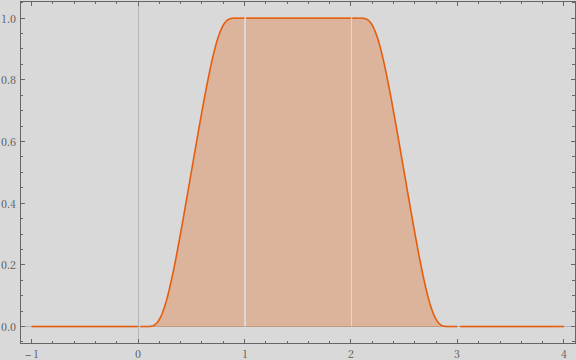
\includegraphics[width=10cm]{construction}
    \caption{Construcción de función de soporte compacto.}
    \label{fig:const}
    \end{figure}
    
    Notar que la misma construcción puede realizarse siguiendo el mismo procedimiento y usando (\ref{eq:trick}), pero con
    alguna otra función $f$ que cumpla $f \in \mathcal{C}^{\infty}(\mathbb{R})$ y $f(0)=0$.

    \end{enumerate}

    Por último, dada una función $\psi \in \mathcal{C}_{C}^{\infty}(\mathbb{R},\mathbb{C})$ con soporte $[a,b] \ \text{y} \ a,b \in \mathbb{R}$, esta puede ser fácilmente extendida a una función $\in \mathcal{C}_{C}^{\infty}(\mathbb{R}^n,\mathbb{C})$, bajo la siguiente construcción:
    \begin{align}
    \Phi(x_1,x_2,\ldots,x_n) = \psi(x_1)\ \psi(x_2)\ \cdots \ \psi(x_n),
    \label{eq:ndbump}
    \end{align}
    cuyo soporte compacto es $[a,b]\times \stackrel{n-2 \text{ veces}}{\ldots} \times [a,b]=[a,b]^n$. En la Figura \ref{fig:3dbump} se muestra tal construcción para la función \textit{bump} clásica en dos variables.
    
    \begin{figure}[htpb!]
    \centering
    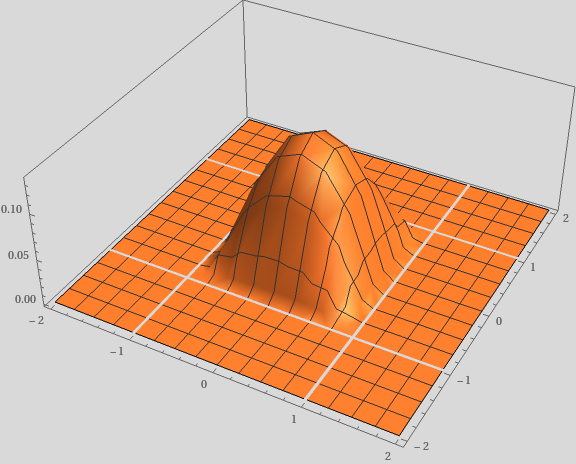
\includegraphics[width=10cm]{3dbump}
    \caption{Gráfico de función \textit{bump} clásica en dos variables.}
    \label{fig:3dbump}
    \end{figure}



    \item[\textsc{Tarea 8.}] Sea $f \in \mathcal{C}_{\downarrow}^{\infty}(\mathbb{R},\mathbb{C})$ una función con soporte compacto $\text{supp}(f) \subset [a,b] \subset [0,T]$ ($0<a<b<T$), con la respectiva prolongación periódica (de periodo $T$)
    \begin{align}
         g(x) = \sum_{n \in \mathbb{Z}} f(x - n T), \ \ \ \ x \in \mathbb{R}.
         \label{eq:prolongacion}
    \end{align} Considerando la norma uniforme $||f||_{\infty} := \sup_{x \in \mathbb{R}} |f(x)|$. Como ya probamos anteriormente (Weierstrass):
    \begin{align*}
        f \in \mathcal{C}_{\downarrow}^{\infty}(\mathbb{R},\mathbb{C}) \Rightarrow 0 \leq ||f||_{\infty} < \infty.
    \end{align*}
    Debido a la construcción de la prolongación periódica (\ref{eq:prolongacion}), se sabe que no existen traslapes entre
    las \textit{copias} de $f$ en los distintos periodos. Entonces:
    \begin{align*}
        ||g||_{\infty} = \sup_{x \in \mathbb{R}} |g(x)| = \sup_{x \in \mathbb{R}} \left|\sum_{n \in \mathbb{Z}} f(x - n T)\right| \stackrel{(\#)}{=} \sup_{x \in \mathbb{R}} |f(x-nT)|\ \ (\forall n \in \mathbb{Z})= \sup_{x \in \mathbb{R}} |f(x)| = ||f||_{\infty} < \infty
    \end{align*}
    donde $(\#)$ es posible, pues como se hizo notar, todas las copias de $f$ son iguales y sin traslapes. Puesto que $||g||_{\infty} < \infty$, se comprueba entonces la convergencia de la serie.




    \item[\textsc{Tarea 9.}] Se analiza cada punto por parte.
    \begin{itemize}
        \item[a,b)] Sea $f \in L^1 \cap L^2$, entonces $\displaystyle \mathcal{F}(f) = \widehat{f}(\omega) = \int_{-\infty}^{\infty} f(t) e^{-i \omega t} dt  \leq \int_{-\infty}^{\infty} |f(t)| dt < \infty$ está bien definido. Luego, notar que aplicando la operación de conjugación se obtiene:
        \begin{align*}
            \overline{\hat{f}(\omega)}=\overline{\int_{-\infty}^{\infty}f(t)e^{-i \omega t}dt}=\int_{-\infty}^{\infty}\overline{f(t)}e^{i\omega t}dt \stackrel{t \rightarrow -t'}{=} \int_{\infty}^{-\infty}\overline{f(-t')}e^{-i \omega t'}(-dt') = \int_{-\infty}^{\infty}\overline{f(-t')}e^{-i \omega t'}dt'.
        \end{align*}
        Sea $g(t)=\overline{f(-t)}$ ($g \in L^1 \cap L^2$ también), entonces $\overline{\hat{f}(\omega)}=\hat{g}(\omega)$. Además, como se demostró anteriormente:
        \begin{align}
            \widehat{f * g}(\omega) = \widehat{f}(\omega)\cdot \widehat{g}(\omega) =  \widehat{f}(\omega)\cdot \overline{\widehat{f}(\omega)} = \left| \widehat{f}(\omega) \right|^2.
        \label{eq:proper}
        \end{align} 
        Luego haciendo uso de (\ref{eq:proper}) se prodece como sigue:
        \begin{align}
       \int_{-\infty}^{\infty}|\widehat{f}(\omega)|^2d\omega & =\left.\int_{-\infty}^{\infty}\widehat{f * g}(\omega)e^{i \omega x}d\omega \right|_{x=0} \\
       & = \mathcal{F}^{-1}(\widehat{f * g})  (0) = (f * g)(0) \\
       & = \int_{-\infty}^{\infty}f(t)g(0-t)dt = \int_{-\infty}^{\infty}f(t)\overline{f(t)}dt  \\
       & = \int_{-\infty}^{\infty}|f(t)|^2dt <  \infty.
        \end{align}
        Esto último prueba los dos puntos: $||f||_2 = ||\widehat{f}||_2$ y que $\widehat{f} \in L^2$.
    \end{itemize}

\end{description}


\bibliographystyle{plain}
\bibliography{referencias}


\end{document}


